%/*% pdflatex -file-line-error -interaction nonstopmode %

\documentclass{article}
\usepackage{graphicx}
\usepackage{amsmath}
\usepackage{amsfonts}
\usepackage{bookmark}
\usepackage{booktabs}
\usepackage{exercises}
\graphicspath{ {./images/quiz2} }
\usepackage{indentfirst}
\usepackage{amsthm}
\usepackage{yhmath}
\usepackage{placeins}
\newcommand*{\oldneg}{\mathord{\sim}}
\newcommand\showdiv[1]{\overline{\smash{)}#1}}
\newcommand\Mydiv[1]{%
\smash{\raise.3ex\hbox{$\big)$}}\mkern-8mu
        \overline{\enspace\strut#1}}
\setlength{\tabcolsep}{5pt}
\theoremstyle{definition}
\newtheorem{definition}{Definition}

\setlength{\parindent}{.5in}
\setlength{\parskip}{12pt}
\renewcommand{\arraystretch}{1}

\title{Quiz 2 (Page 150)}
\begin{document}
\maketitle

\section*{1}
We can use the rational roots theorem to determine that all the possible real zeros of this function are:
\[ \pm 1,\pm 2,\pm 5, \pm 6, \pm 10, \pm 15, \pm 30 \]
Using a calculator, we can see that $2$ is one such solution. By the Factor Theorem, we know that $x-2$ is a factor of the polynomial. 
Therefore, we can use synthetic division to find the other factor:
\begin{center}
\begin{tabular}{l|rrrr}
	$2$ & $1$ & $-4$ & $-11$ & $30$ \\
	& & $2$ & $-4$ & $-30$ \\
	\cmidrule{2-5}
	& $1$ & $-2$ & $-15$ & $0$
\end{tabular}
\end{center}
meaning the other factor of the polynomial is \[ x^2-2x-15=(x-5)(x+3) \] We can therefore conclude that the three zeros of this polynomial are 
$2$, $5$, $-3$. This matches up with the fundemental theorem of algebra, which says that this polynomial (of degree 3) has exactly 3 zeros.

\section*{2}
We can use the rational roots theorem to determine all of the possible real zeros. Using a calculator, we can determine that $5$ is one such zero.
Thus, by the factor theorem, we know that $x-5$ is a factor of the polynomial. We can then use synthetic division to find the other factor:
\begin{center}
\begin{tabular}{l|rrrrr}
	$5$ & $2$ & $-2$ & $-49$ & $9$ & $180$ \\
	& & $10$ & $40$ & $-45$ & $-180$ \\
	\cmidrule{2-6}
	& $2$ & $8$ & $-9$ & $-36$ & $0$
\end{tabular}
\end{center}
meaning we can conclude that $2x^3+8x^2-9x-36$ is the other factor of the polynomial. We can use the rational roots theorem again, and determine 
a zero of this function is $-4$. Using the same process, we can use synthetic division to find the other factor:
\begin{center}
\begin{tabular}{l|rrrr}
	$-4$ & $2$ & $8$ & $-9$ & $-36$ \\
	& & $-8$ & $0$ & $36$ \\
	\cmidrule{2-5}
	& $2$ & $0$ & $-9$ & $0$
\end{tabular}
\end{center}
meaning the other factor is $2x^2-9$. The zeros of this function are 
\[ x=\pm\frac{3\sqrt{2}}{2} \] Meaning we can conclude that the zeros of 
\[ 2x^4-2x^3-49x^2+9x+180 \] are $5$, $-4$, $\pm\frac{3\sqrt{2}}{2}$. This matches up with the fundemental theorem of algebra, which says that 
this polynomial (of degree 4) has exactly 4 zeros.

\section*{3}
\[ f(x)=(x+4)(x+1)(x-2)=(x^2+5x+4)(x-2)=x^3+3x^2-6x-8 \]

\section*{4}
By the complex conjugates theorem we know that if $1+i$ is a zero of $f$ (which has rational coefficients), then so is $1-i$:
\[ f(x)=(x-4)(x-(1+i))(x-(1-i))=(x-4)(x-1-i)(x-1+i) \]

\section*{5}
By the irrational conjugates theorem, we know that if $7+\sqrt{2}$ is a zero of $f$ (which has rational coefficients), then so is $7-\sqrt{2}$:
\[ f(x)=(x+3)(x-5)(x-(7+\sqrt{2}))(x-(7-\sqrt{2})) \]

\section*{6}
By the irrational conjugates theorem, we know that if $3-\sqrt{6}$ is a zero of $f$ (which has rational coefficients), then so is $3+\sqrt{6}$. 
By the complex conjugates theorem, we 
know that if $-2i$ is a zero of $f$, then so is $2i$:
\[ f(x)=(x-1)(x+2i)(x-2i)(x-(3-\sqrt{6}))(x-(3+\sqrt{6})) \]

\section*{7}
We know that the real zeros of $f$ are $3,2$ and $-2$. Because this is a polynomial function of odd degree with a negative leading coefficient 
($-1$), we know that $f(x)\rightarrow +\infty$ as $x\rightarrow -\infty$, and $f(x)\rightarrow -\infty$ as $x\rightarrow +\infty$. Because 
every zero of the function, when put into its factored form, is raised to an odd degree, we know that the graph intersects these points. This is sufficient 
information to draw a graph of this function:
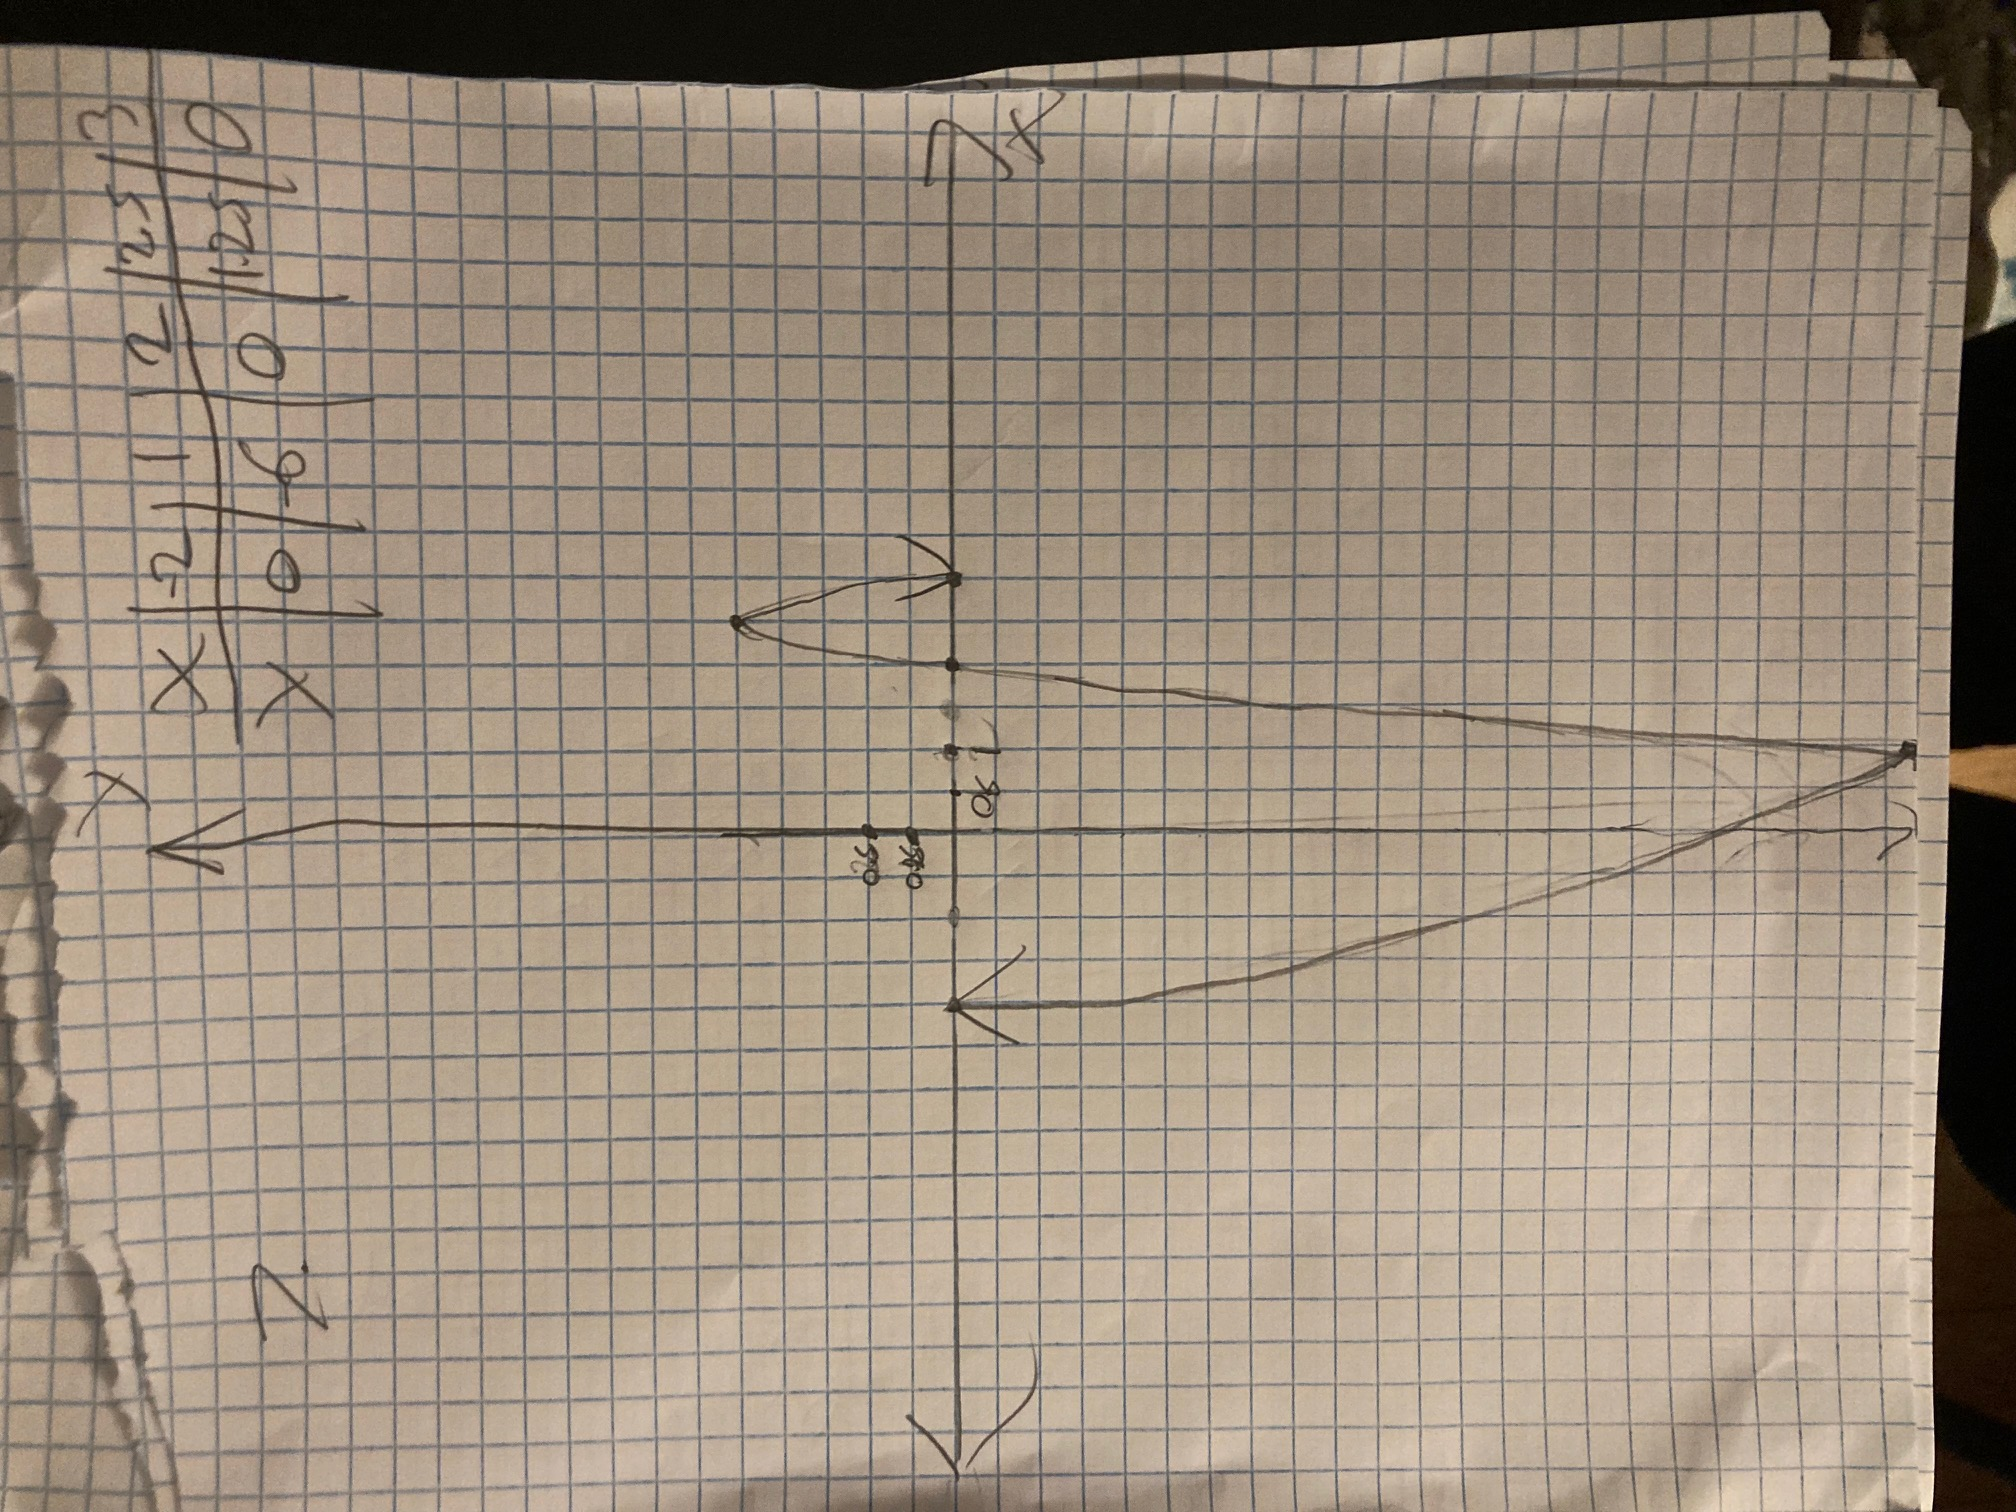
\includegraphics[width = 4in, height = 4in, angle = -90]{picture7}

\section*{8}
We know that the real zeros of $f$ are $1,-1$ and $4$. Because this is a polynomial function of odd degree with a positive leading coefficient ($3$), 
we know that $f(x)\rightarrow +\infty$ as $x\rightarrow +\infty$ and $f(x)\rightarrow -\infty$ as $x\rightarrow -\infty$. Because the factor of every zero 
of the function is raised to an odd degree (1), we know that the graph intersects these points. This is sufficient information to draw a graph of 
this function:
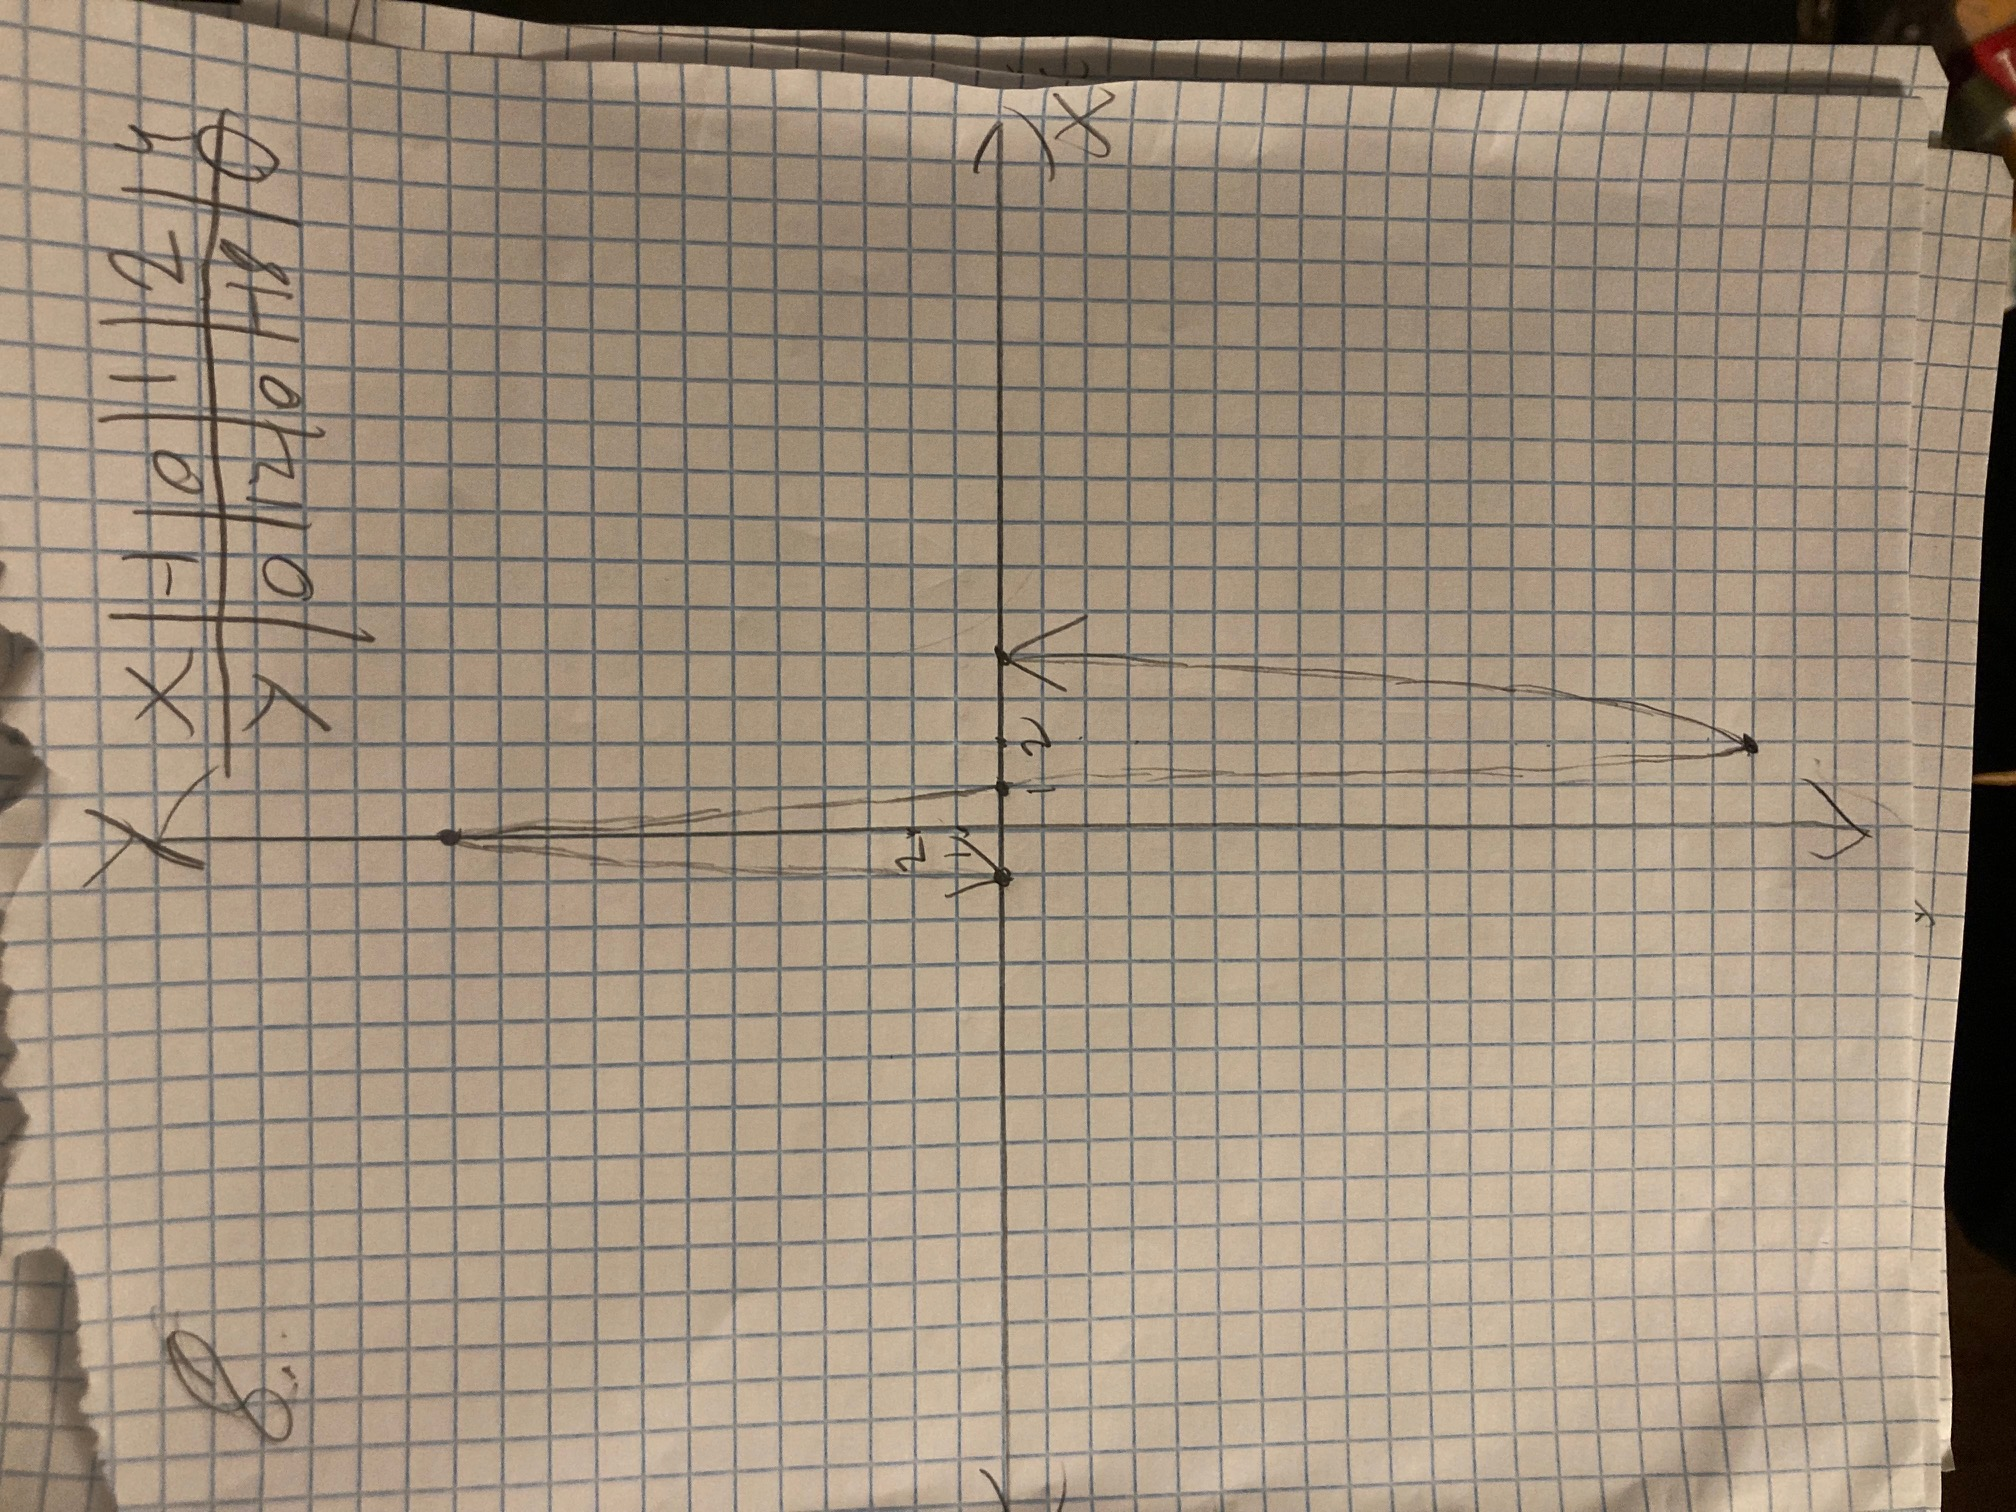
\includegraphics[width = 4in, height = 4in, angle = -90]{picture8}

\section*{9}
We know that the real zeros of $f$ are $0,4,1$ and $-2$. Because this is a polynomial function of even degree with a positive leading coefficient ($1$), 
we know that $f(x)\rightarrow +\infty$ as $x\rightarrow \pm\infty$. Because the factor of every zero of the function is raised to an odd degree (1), 
we know that the graph intersects these points:
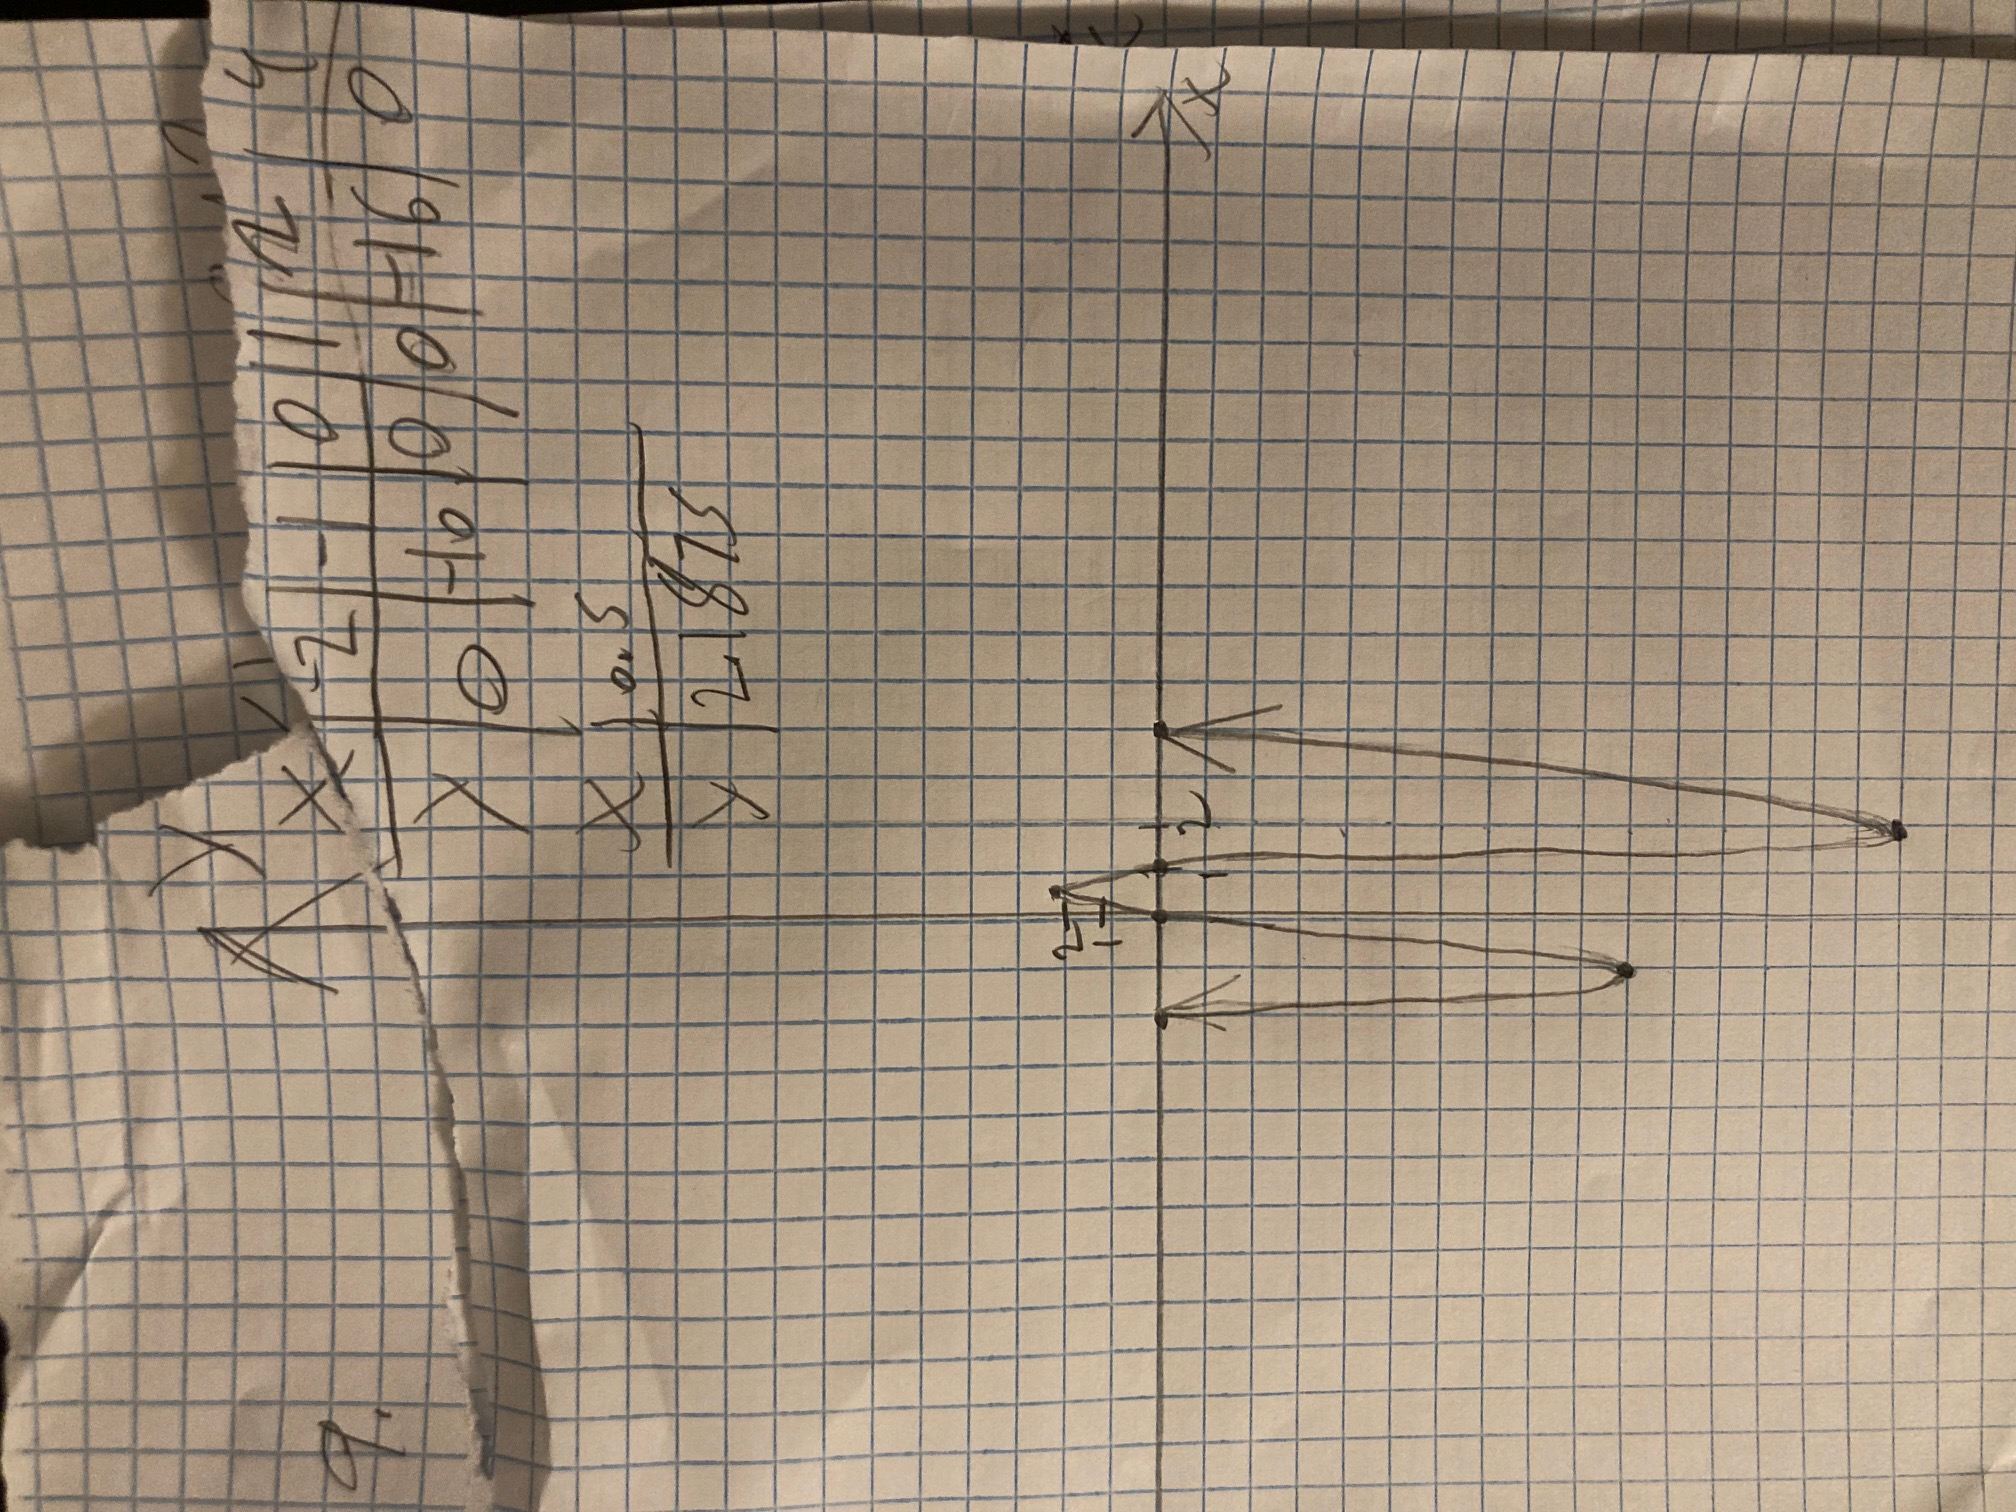
\includegraphics[width = 4in, height = 4in, angle = -90]{picture9}

\section*{10}
We know that the real zeros of $f$ are $3,-2$ and $-3$. Because this is a polynomial function of odd degree with a positive leading coefficient ($1$), 
we know that $f(x)\rightarrow +\infty$ as $x\rightarrow +\infty$ and $f(x)\rightarrow -\infty$ as $x\rightarrow -\infty$. Because the factors $x+2$ and 
$x+3$ of the function are raised to an even degree, we know that the graph of the function is tangent to these points:
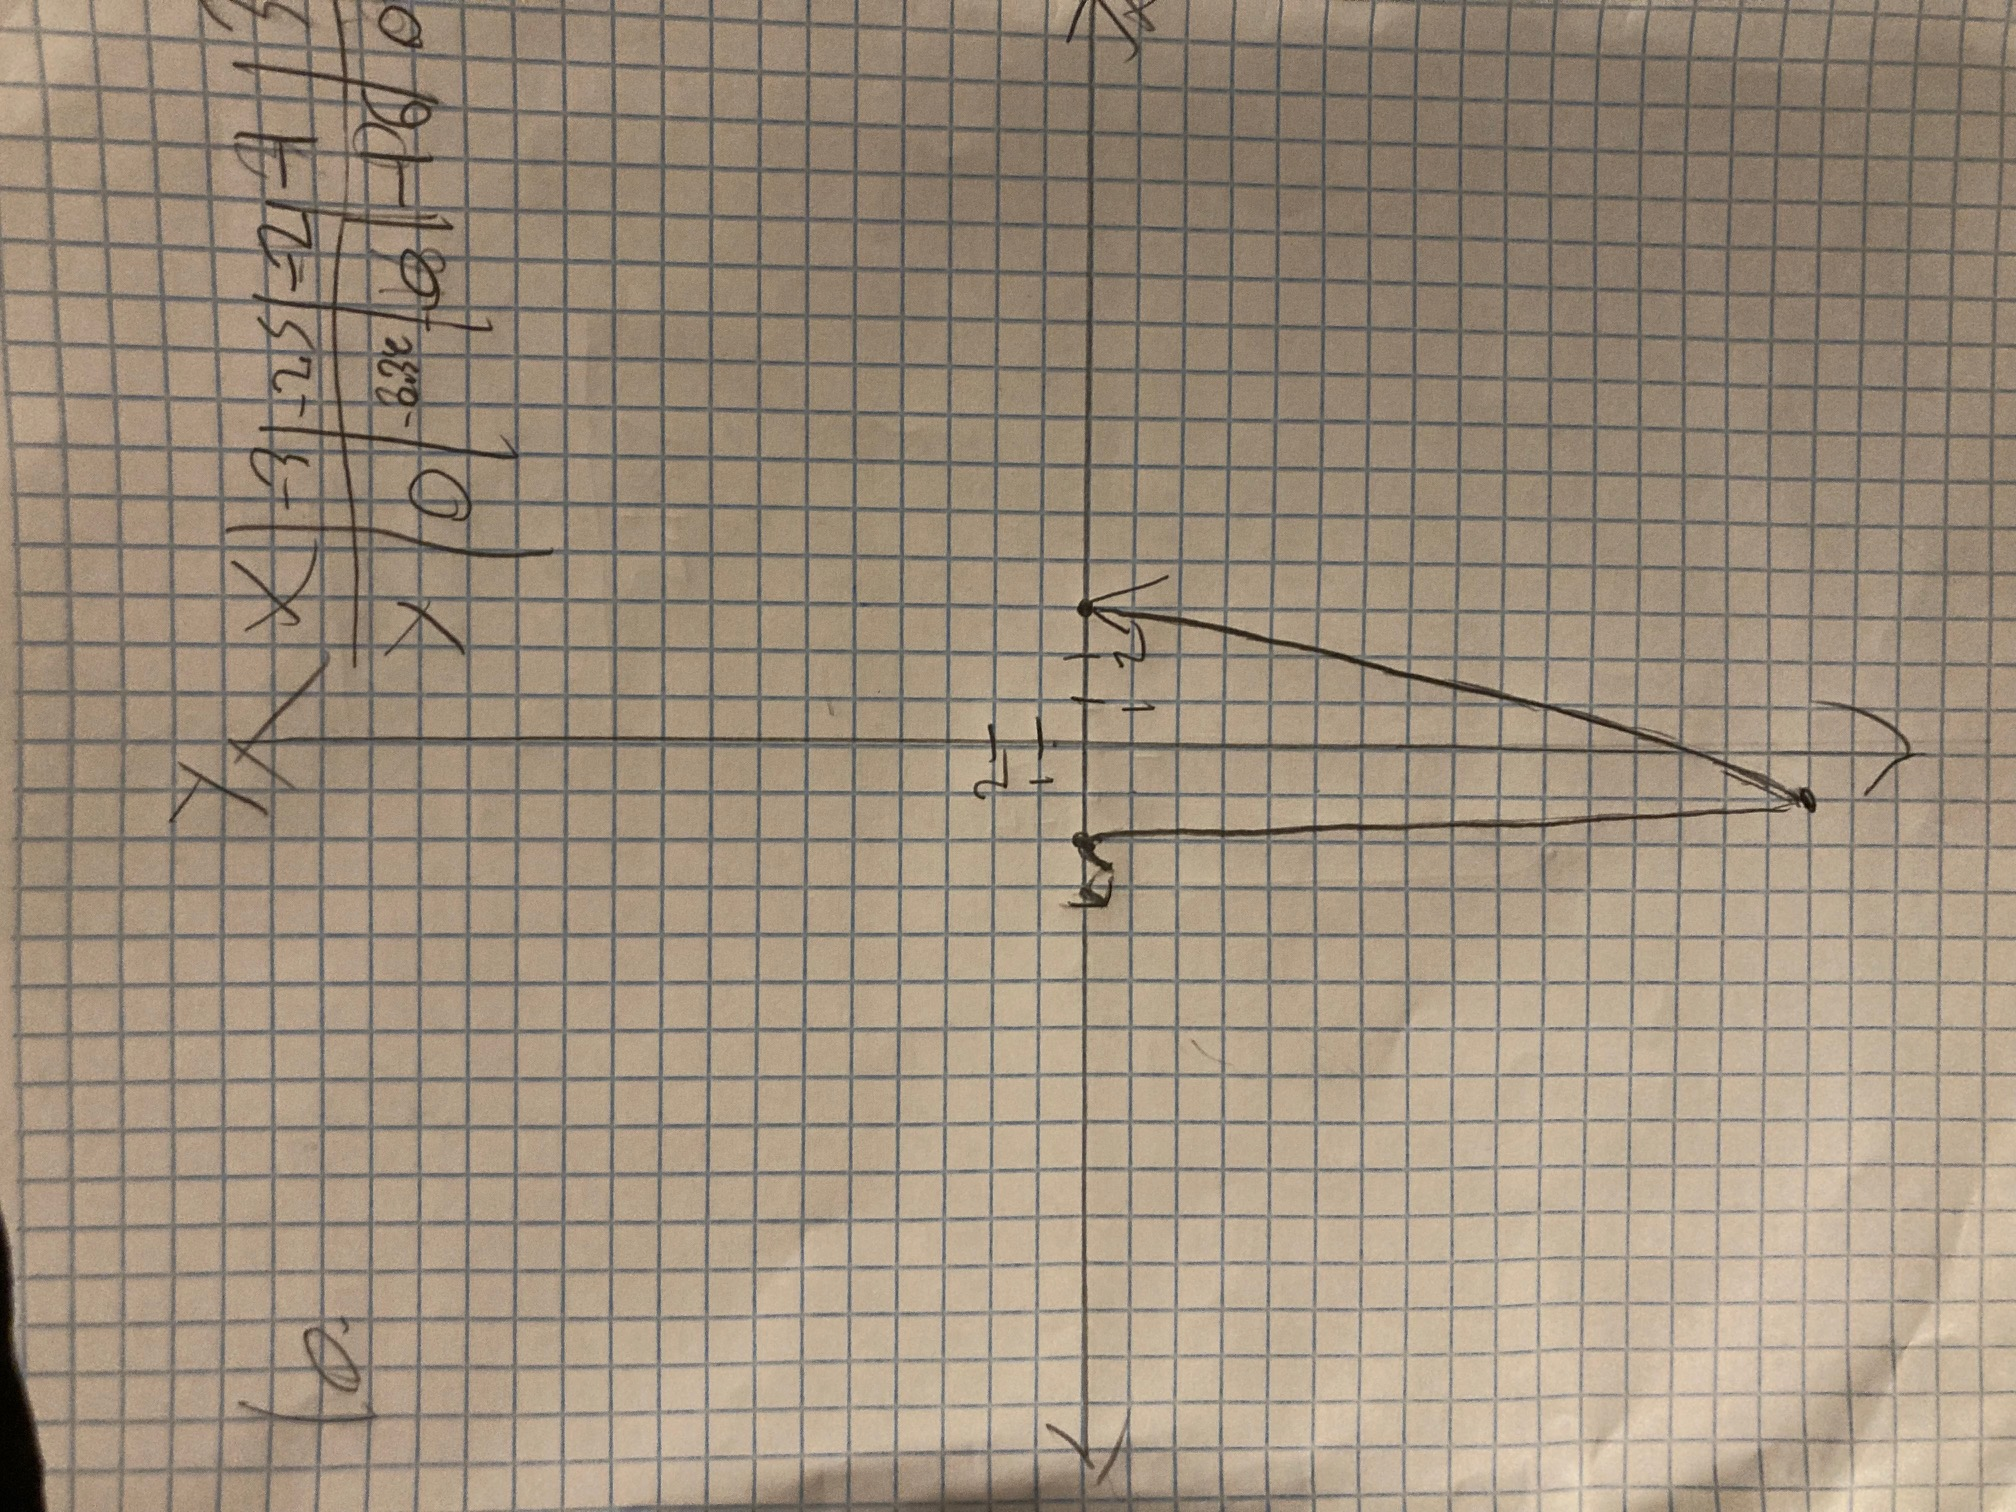
\includegraphics[width = 4in, height = 4in, angle = -90]{picture10}

\end{document}
